\section{The Admission Setting}
\label{sec:construction}
\label{sec:benchmarks}

Our setting makes one useful concept compete with passage concepts
for a fixed number of memory slots. Each episode contains a passage,
an ordered candidate set, utility labels, and a future question with
its answer (Figure~\ref{fig:episode}). With two memory slots, the city
in Figure~\ref{fig:episode} competes with the elevator, gift shop, and
scenery. Only the passage and candidates reach the admission policy.

\subsection{Episodes}

Each episode centers on a useful concept: information linking the
passage to a future answer, which the generator calls the
\emph{bridge}. \textbf{Decoupled} requires two inference steps: recover
the useful concept from the passage, then combine it with general
knowledge to answer the future question. GPT-4.1 generates a passage
about a named person, together with the useful concept, question, and
answer.
The answer is excluded from the passage and candidate set, while the
question connects to the passage through the person's name.

The generator assigns gold utility labels using the useful concept and
the question it writes: positive for the useful concept, and negative
for vivid surface distractors and neutral passage concepts. Rule-based
filters check candidate strings, exclusion of the useful concept and
answer, and question overlap, while deduplication removes repeated
concepts. A blind alias filter checks that recovering the useful
concept still leaves an inference to the answer
(App.~\ref{app:benchmarks}).

\begin{figure*}[t]
\centering
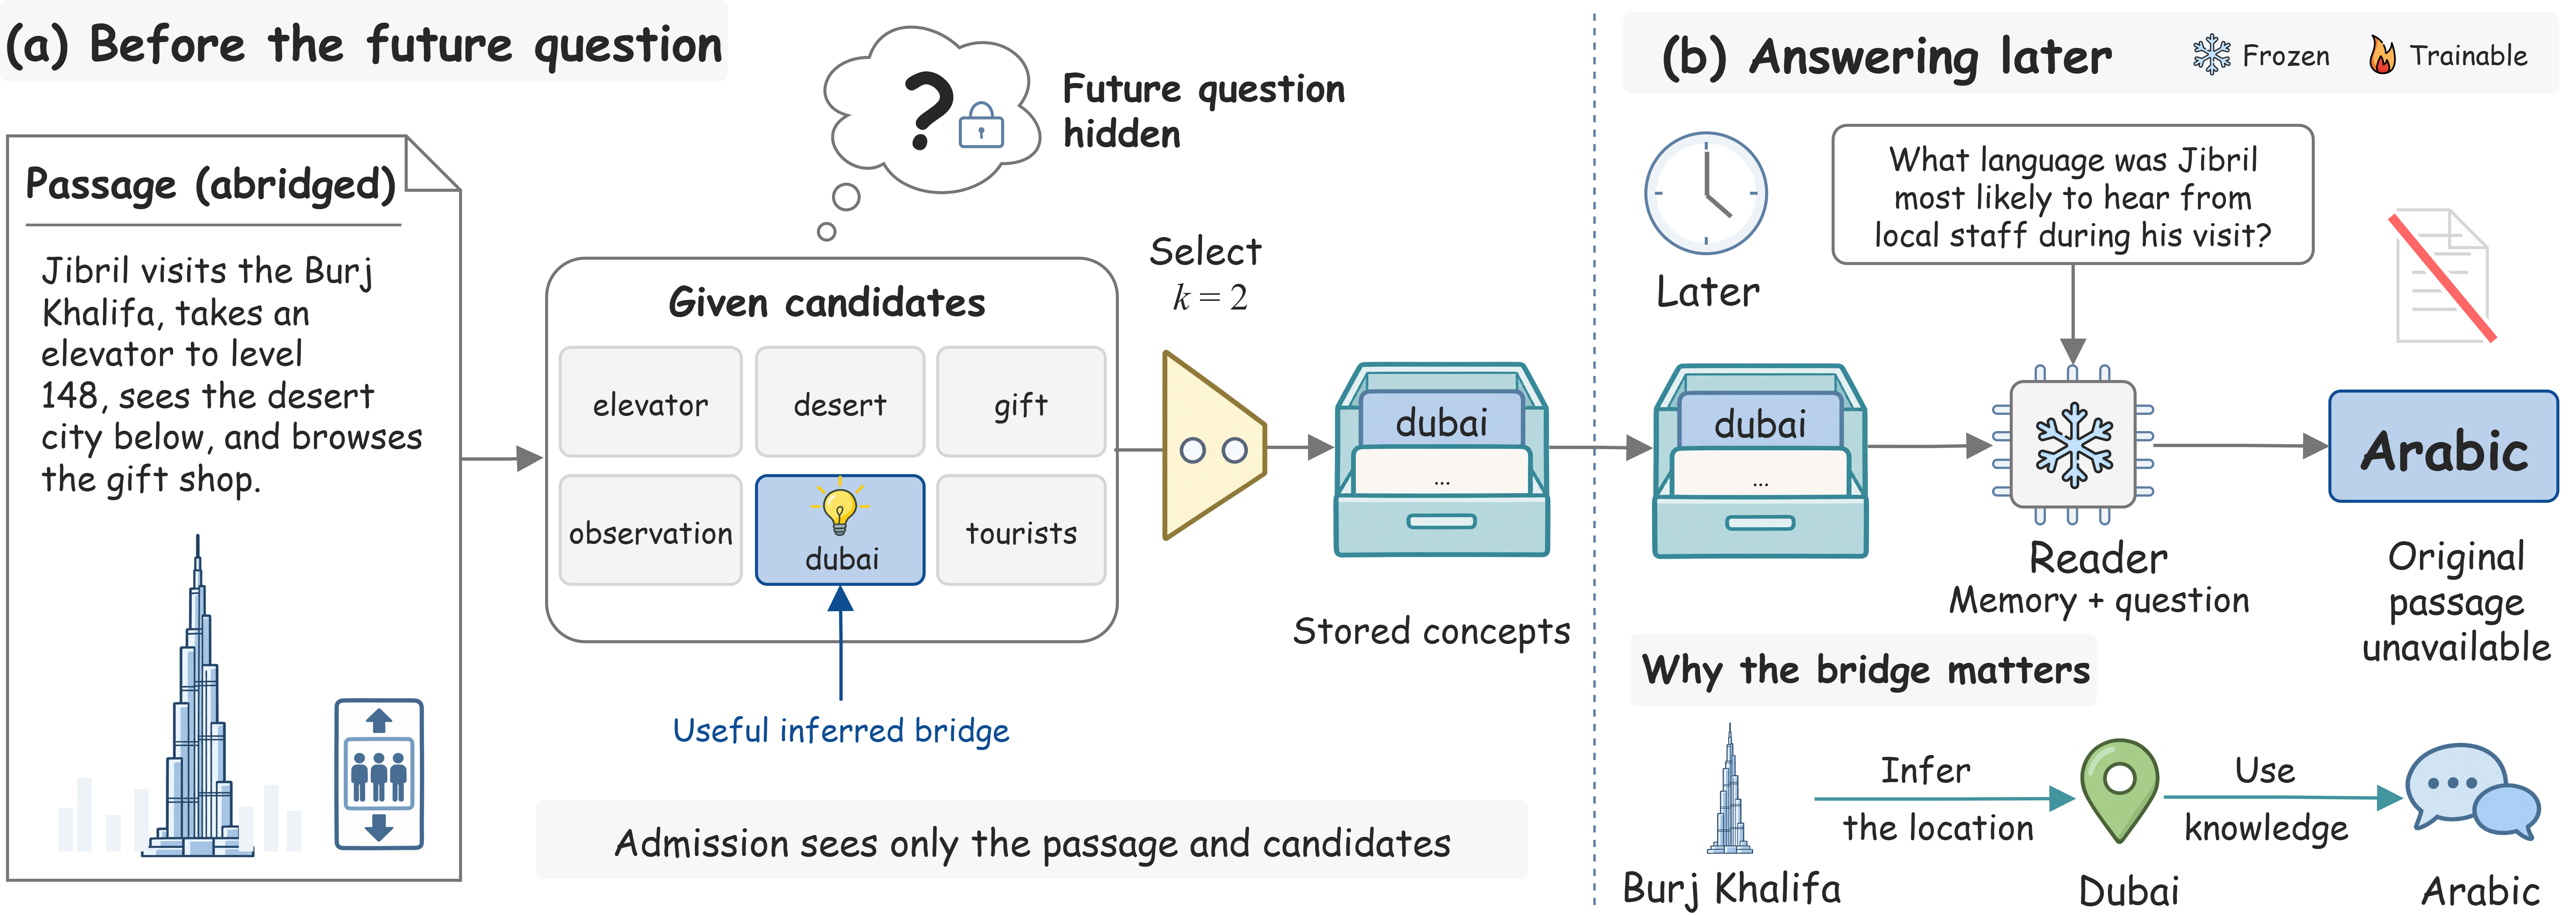
\includegraphics[width=\textwidth]{figures/fig3.png}
\caption{An abridged admission episode. (a) Before the question arrives, the policy sees only the passage and candidates, storing $k=2$ concepts. The useful concept, \emph{dubai}, is the sole unstated candidate. (b) Later, the frozen reader answers from stored concepts without the passage. Figure~\ref{fig:examples} gives the full episode.}
\label{fig:episode}
\end{figure*}

\textbf{Explicit} states the useful concept in the passage.
\textbf{Compositional} requires a multi-hop answer and permits passage
anchors in the question. A \textbf{held-out set} and a
\textbf{test set} repeat the Decoupled construction with new passages
and useful concepts absent from the training episodes. The test set
also excludes the held-out set's contexts.

\subsection{Candidate Pools and Controls}

The pools and controls separate the effects of passage mention,
candidate competition, context, generator, and useful-concept category.
The \textbf{original pool} is the generator's candidate list for each
test-set episode: 1,607 candidates, 4.43 per episode.
Each pool and control preserves each episode's future question,
answer, and original utility labels; added candidates receive
negative labels.

\paragraph{Mention and position.}
These controls isolate the named concept and sentence position.
The \textbf{stated-bridge control} appends \emph{The passage also
mentions bridge.} The \textbf{position control} places that sentence
before the passage, whereas the \textbf{distractor-named control}
substitutes a distractor for the bridge in the appended sentence.

\paragraph{Competition for memory.}
Our main evaluation pool, the \textbf{statedness-balanced pool}, uses
the 363 test-set episodes in fixed order. Odd positions, counted from
the first episode, keep the passage unchanged; even positions append
\emph{The passage also mentions bridge.} with \emph{bridge} replaced
by the useful concept. Under the case-insensitive stem rule, the
stated-concept condition contains 190 episodes: all even positions
and 9 odd positions whose original passages already match the useful
concept. The unstated-concept condition contains 173 episodes, all
at odd positions.

Every episode retains its original candidates, including stated
distractors, and adds the first four (odd positions) or three (even
positions) additional unstated candidates, in order, from the pool
with unstated distractors described below. Position alone determines
the naming sentence and distractor count, with no sampling
(App.~\ref{app:pools}).

The resulting 363 episodes average 7.93 candidates, with useful
concepts accounting for 13.3\% of stated candidates and 12.0\% of
unstated candidates. A statedness-only rule ranks near chance, with
pooled AUC of 0.515 and within-episode AUC of 0.516.

The \textbf{naming-balanced pool} names four candidates in every
episode using five sentence templates at varying positions; named
candidates are useful 12.5\% of the time, against a 12.6\% base rate.

Each pool balances one cue and leaves the other imbalanced in the
opposite direction: in the statedness-balanced pool, the added naming
sentence always names the useful concept, whereas in the
naming-balanced pool, stated candidates are more often distractors.

Two further pools start from the original pool, increasing the
alternatives admission must rank for the same memory budget.
The \textbf{pool with unstated distractors} adds four confusable
concepts from the useful concept's semantic category. An LLM proposes these
concepts, which are filtered for absence from the passage and
original pool. The \textbf{enlarged pool} adds further concepts from
other episodes, reaching 12.41 candidates on average.

\paragraph{Context, generator, and useful-concept category.}
These controls test whether admission depends on the episode's own
passage, the generator, or the kind of useful concept.
\textbf{Passage replacement} replaces each passage with another
episode's passage while retaining its candidates and labels.
The \textbf{paired-passage set} pairs test-set episodes that
contain the same candidates in different orders while each retains
its passage, future question, and useful concept
(\S\ref{sec:ablations}, App.~\ref{app:teacherreadout}).
The \textbf{alternate-generator set} uses GPT-4o to write episodes
with an unstated useful concept. The \textbf{entity-bridge set} uses
GPT-5.6 to place a named-entity bridge among scene-object distractors
(App.~\ref{app:replications}).
